\documentclass[tikz]{standalone}
\begin{document}
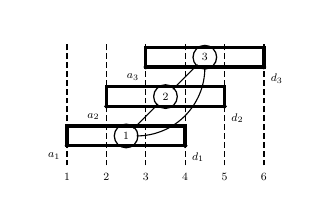
\begin{tikzpicture}[scale=0.5,transform shape]
\clip (0,0) rectangle (7.000000,4.000000);
%%
\definecolor{c1}{rgb}{0.70,0.25,0.25}%
\definecolor{c2}{rgb}{0.25,0.70,0.25}%
\definecolor{c3}{rgb}{0.25,0.25,0.70}%
%
{\footnotesize

% Marking point A1 by circle
\draw [line width=0.016cm] (1.000000,1.000000) circle (0.040000);%
\draw (0.930000,0.930000) node [anchor=north east] { $a_1$ };%

% Marking point D1 by circle
\draw [line width=0.016cm] (4.000000,1.000000) circle (0.040000);%
\draw (4.070000,0.930000) node [anchor=north west] { $d_1$ };%

% Marking point A2 by circle
\draw [line width=0.016cm] (2.000000,2.000000) circle (0.040000);%
\draw (1.930000,1.930000) node [anchor=north east] { $a_2$ };%

% Marking point D2 by circle
\draw [line width=0.016cm] (5.000000,2.000000) circle (0.040000);%
\draw (5.070000,1.930000) node [anchor=north west] { $d_2$ };%

% Marking point A3 by circle
\draw [line width=0.016cm] (3.000000,3.000000) circle (0.040000);%
\draw (2.930000,2.930000) node [anchor=north east] { $a_3$ };%

% Marking point D3 by circle
\draw [line width=0.016cm] (6.000000,3.000000) circle (0.040000);%
\draw (6.070000,2.930000) node [anchor=north west] { $d_3$ };%

% Printing text at point t1
\draw (1.000000,0.400000) node [anchor=north] { $1$ };%

% Printing text at point t2
\draw (2.000000,0.400000) node [anchor=north] { $2$ };%

% Printing text at point t3
\draw (3.000000,0.400000) node [anchor=north] { $3$ };%

% Printing text at point t4
\draw (4.000000,0.400000) node [anchor=north] { $4$ };%

% Printing text at point t5
\draw (5.000000,0.400000) node [anchor=north] { $5$ };%

% Printing text at point t6
\draw (6.000000,0.400000) node [anchor=north] { $6$ };%

% Printing text at point b1
%\color{red}
%\draw (0.500000,1.250000) node  { $1$ };%

% Printing text at point b2
%\color{green}
%\draw (0.500000,2.250000) node  { $3$ };%

% Printing text at point b3
%\color{blue}
%\draw (0.500000,3.250000) node  { $2$ };%

% Filling rectangle left-bottom: A1 right-top: C1
%\color{red}% 
%\fill[red,fill opacity=0.5] (1.000000,1.000000) -- (4.000000,1.000000) -- (4.000000,1.500000) -- (1.000000,1.500000);%
\color{black}% 
\draw[black,very thick] (1,1) rectangle (4,1.5);%marking borders
\draw [line width=0.016cm] (2.5cm,1.25cm) circle (0.30cm);%
\node (1) at (2.5cm,1.25cm) [circle] {$1$};


% Filling rectangle left-bottom: A2 right-top: C2
%\color{green}%  
%\fill[green,fill opacity=0.5] (2.000000,2.000000) -- (5.000000,2.000000) -- (5.000000,2.500000) -- (2.000000,2.500000);%
\color{black}% 
\draw[black,very thick] (2,2) rectangle (5,2.5);%marking borders
\draw [line width=0.016cm] (3.5cm,2.25cm) circle (0.30cm);%
\node (2) at (3.5cm,2.25cm) [circle] {$2$};

% Filling rectangle left-bottom: A3 right-top: C3
%\color{blue}% 
%\fill[blue,fill opacity=0.5] (3.000000,3.000000) -- (6.000000,3.000000) -- (6.000000,3.500000) -- (3.000000,3.500000);%
\color{black}% 
\draw[black,very thick] (3,3) rectangle (6,3.5);%marking borders
\draw [line width=0.016cm] (4.5cm,3.25cm) circle (0.30cm);%
\node (3) at (4.5cm,3.25cm) [circle] {$3$};

% Drawing segment B1 U1
\draw [line width=0.016cm] (1.000000,0.500000) -- (1.000000,0.650000);%
\draw [line width=0.016cm] (1.000000,0.725000) -- (1.000000,0.875000);%
\draw [line width=0.016cm] (1.000000,0.950000) -- (1.000000,0.960000);%
\draw [line width=0.016cm] (1.000000,1.040000) -- (1.000000,1.100000);%
\draw [line width=0.016cm] (1.000000,1.175000) -- (1.000000,1.325000);%
\draw [line width=0.016cm] (1.000000,1.400000) -- (1.000000,1.550000);%
\draw [line width=0.016cm] (1.000000,1.625000) -- (1.000000,1.775000);%
\draw [line width=0.016cm] (1.000000,1.850000) -- (1.000000,2.000000);%
\draw [line width=0.016cm] (1.000000,2.075000) -- (1.000000,2.225000);%
\draw [line width=0.016cm] (1.000000,2.300000) -- (1.000000,2.450000);%
\draw [line width=0.016cm] (1.000000,2.525000) -- (1.000000,2.675000);%
\draw [line width=0.016cm] (1.000000,2.750000) -- (1.000000,2.900000);%
\draw [line width=0.016cm] (1.000000,2.975000) -- (1.000000,3.125000);%
\draw [line width=0.016cm] (1.000000,3.200000) -- (1.000000,3.350000);%
\draw [line width=0.016cm] (1.000000,3.425000) -- (1.000000,3.575000);%

% Drawing segment B2 U2
\draw [line width=0.016cm] (2.000000,0.500000) -- (2.000000,0.650000);%
\draw [line width=0.016cm] (2.000000,0.725000) -- (2.000000,0.875000);%
\draw [line width=0.016cm] (2.000000,0.950000) -- (2.000000,1.100000);%
\draw [line width=0.016cm] (2.000000,1.175000) -- (2.000000,1.325000);%
\draw [line width=0.016cm] (2.000000,1.400000) -- (2.000000,1.550000);%
\draw [line width=0.016cm] (2.000000,1.625000) -- (2.000000,1.775000);%
\draw [line width=0.016cm] (2.000000,1.850000) -- (2.000000,2.000000);%
\draw [line width=0.016cm] (2.000000,2.075000) -- (2.000000,2.225000);%
\draw [line width=0.016cm] (2.000000,2.300000) -- (2.000000,2.450000);%
\draw [line width=0.016cm] (2.000000,2.525000) -- (2.000000,2.675000);%
\draw [line width=0.016cm] (2.000000,2.750000) -- (2.000000,2.900000);%
\draw [line width=0.016cm] (2.000000,2.975000) -- (2.000000,3.125000);%
\draw [line width=0.016cm] (2.000000,3.200000) -- (2.000000,3.350000);%
\draw [line width=0.016cm] (2.000000,3.425000) -- (2.000000,3.575000);%

% Drawing segment B3 U3
\draw [line width=0.016cm] (3.000000,0.500000) -- (3.000000,0.650000);%
\draw [line width=0.016cm] (3.000000,0.725000) -- (3.000000,0.875000);%
\draw [line width=0.016cm] (3.000000,0.950000) -- (3.000000,0.960000);%
\draw [line width=0.016cm] (3.000000,1.040000) -- (3.000000,1.100000);%
\draw [line width=0.016cm] (3.000000,1.175000) -- (3.000000,1.325000);%
\draw [line width=0.016cm] (3.000000,1.400000) -- (3.000000,1.550000);%
\draw [line width=0.016cm] (3.000000,1.625000) -- (3.000000,1.775000);%
\draw [line width=0.016cm] (3.000000,1.850000) -- (3.000000,1.960000);%
\draw [line width=0.016cm] (3.000000,2.075000) -- (3.000000,2.225000);%
\draw [line width=0.016cm] (3.000000,2.300000) -- (3.000000,2.450000);%
\draw [line width=0.016cm] (3.000000,2.525000) -- (3.000000,2.675000);%
\draw [line width=0.016cm] (3.000000,2.750000) -- (3.000000,2.900000);%
\draw [line width=0.016cm] (3.000000,2.975000) -- (3.000000,3.125000);%
\draw [line width=0.016cm] (3.000000,3.200000) -- (3.000000,3.350000);%
\draw [line width=0.016cm] (3.000000,3.425000) -- (3.000000,3.575000);%

% Drawing segment B4 U4
\draw [line width=0.016cm] (4.000000,0.500000) -- (4.000000,0.650000);%
\draw [line width=0.016cm] (4.000000,0.725000) -- (4.000000,0.875000);%
\draw [line width=0.016cm] (4.000000,0.950000) -- (4.000000,1.100000);%
\draw [line width=0.016cm] (4.000000,1.175000) -- (4.000000,1.325000);%
\draw [line width=0.016cm] (4.000000,1.400000) -- (4.000000,1.550000);%
\draw [line width=0.016cm] (4.000000,1.625000) -- (4.000000,1.775000);%
\draw [line width=0.016cm] (4.000000,1.850000) -- (4.000000,2.000000);%
\draw [line width=0.016cm] (4.000000,2.075000) -- (4.000000,2.225000);%
\draw [line width=0.016cm] (4.000000,2.300000) -- (4.000000,2.450000);%
\draw [line width=0.016cm] (4.000000,2.525000) -- (4.000000,2.675000);%
\draw [line width=0.016cm] (4.000000,2.750000) -- (4.000000,2.900000);%
\draw [line width=0.016cm] (4.000000,2.975000) -- (4.000000,3.125000);%
\draw [line width=0.016cm] (4.000000,3.200000) -- (4.000000,3.350000);%
\draw [line width=0.016cm] (4.000000,3.425000) -- (4.000000,3.575000);%

% Drawing segment B5 U5
\draw [line width=0.016cm] (5.000000,0.500000) -- (5.000000,0.650000);%
\draw [line width=0.016cm] (5.000000,0.725000) -- (5.000000,0.875000);%
\draw [line width=0.016cm] (5.000000,0.950000) -- (5.000000,1.100000);%
\draw [line width=0.016cm] (5.000000,1.175000) -- (5.000000,1.325000);%
\draw [line width=0.016cm] (5.000000,1.400000) -- (5.000000,1.550000);%
\draw [line width=0.016cm] (5.000000,1.625000) -- (5.000000,1.775000);%
\draw [line width=0.016cm] (5.000000,1.850000) -- (5.000000,1.960000);%
\draw [line width=0.016cm] (5.000000,2.075000) -- (5.000000,2.225000);%
\draw [line width=0.016cm] (5.000000,2.300000) -- (5.000000,2.450000);%
\draw [line width=0.016cm] (5.000000,2.525000) -- (5.000000,2.675000);%
\draw [line width=0.016cm] (5.000000,2.750000) -- (5.000000,2.900000);%
\draw [line width=0.016cm] (5.000000,3.040000) -- (5.000000,3.125000);%
\draw [line width=0.016cm] (5.000000,3.200000) -- (5.000000,3.350000);%
\draw [line width=0.016cm] (5.000000,3.425000) -- (5.000000,3.575000);%

% Drawing segment B6 U6
\draw [line width=0.016cm] (6.000000,0.500000) -- (6.000000,0.650000);%
\draw [line width=0.016cm] (6.000000,0.725000) -- (6.000000,0.875000);%
\draw [line width=0.016cm] (6.000000,0.950000) -- (6.000000,1.100000);%
\draw [line width=0.016cm] (6.000000,1.175000) -- (6.000000,1.325000);%
\draw [line width=0.016cm] (6.000000,1.400000) -- (6.000000,1.550000);%
\draw [line width=0.016cm] (6.000000,1.625000) -- (6.000000,1.775000);%
\draw [line width=0.016cm] (6.000000,1.850000) -- (6.000000,2.000000);%
\draw [line width=0.016cm] (6.000000,2.075000) -- (6.000000,2.225000);%
\draw [line width=0.016cm] (6.000000,2.300000) -- (6.000000,2.450000);%
\draw [line width=0.016cm] (6.000000,2.525000) -- (6.000000,2.675000);%
\draw [line width=0.016cm] (6.000000,2.750000) -- (6.000000,2.900000);%
\draw [line width=0.016cm] (6.000000,2.975000) -- (6.000000,3.125000);%
\draw [line width=0.016cm] (6.000000,3.200000) -- (6.000000,3.350000);%
\draw [line width=0.016cm] (6.000000,3.425000) -- (6.000000,3.575000);%
\color{black}

\path[-] (1) edge (2);
\path[-] (2) edge (3);
\path[-] (1) edge [out=0, in=-90] (3);

}
\end{tikzpicture}
\end{document}
